\section{The models}

To systematically evaluate the effects of geometric changes, the models were developed with varying levels of complexity, incorporating different numbers of degrees of freedom. Both models represent idealized TCPC geometries and share the same labeling convention for inlets and outlets. 

The inlets are denoted as $\Gamma^{\text{N}}_{\text{in}}$ (representing the superior vena cava at the top) and $\Gamma^{\text{S}}_{\text{in}}$ (representing the inferior vena cava with the conduit at the bottom). Similarly, the outlets are labeled as $\Gamma^{\text{W}}_{\text{out}}$ (representing the left part of the pulmonary artery) and $\Gamma^{\text{E}}_{\text{out}}$ (representing the right part of the pulmonary artery).
The shared geometric framework and boundary labels, is illustrated in Figure~\ref{fig:junction schema}. The dimensions of cylindrical segments forming the simplified junction along with their corresponding abbreviations are presented in Table~\ref{tab:tcpc dims}.


\begin{figure}[H]
	\centering
	\vspace{2mm}
	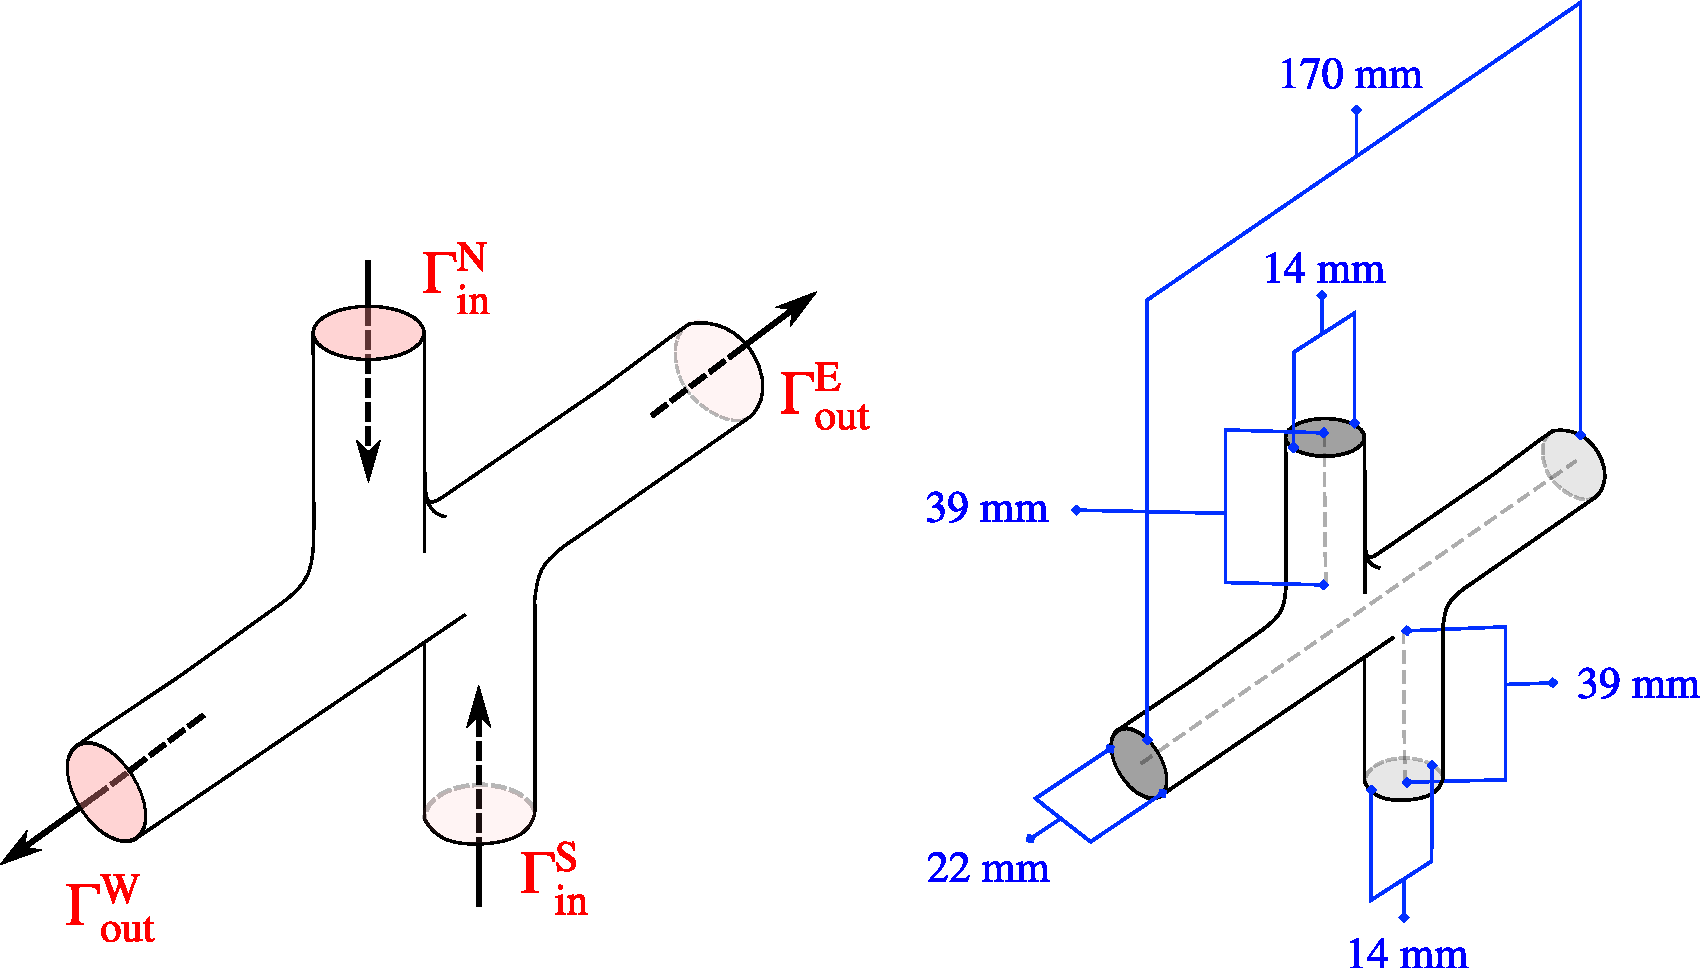
\includegraphics[width=0.99\textwidth]{figures/3d-tcpc-schema-combined.pdf}
	\vspace{7mm}
	\caption{Schematic representation of the idealized TCPC geometry. The labeled inlets ($\Gamma^{\text{N}}_{\text{in}}$, $\Gamma^{\text{S}}_{\text{in}}$) and outlets ($\Gamma^{\text{W}}_{\text{out}}$, $\Gamma^{\text{E}}_{\text{out}}$), directions of inflows and outflows, and the dimensions of the cylindrical segments forming the junction are illustrated.}
	\label{fig:junction schema}
\end{figure}

\bgroup
\centering
\vspace{4mm}
\setlength\tabcolsep{3mm}
\def\arraystretch{1.7}%
\begin{tabular}{|l|l|c|c|}
	\hline
	Segment & Abbreviation & Length & Diameter \\ \hline
	Inferior vena cava 	& IVC 	&      39 mm        &     14 mm    \\ 
	Superior vena cava  & SVC 	&      39 mm     	&     14 mm     \\ 
	Pulmonary artery 	& PA 	&      170 mm     	&     22 mm     \\  \hline
\end{tabular}
\vspace{2mm}
\captionof{table}{Dimensions and abbreviations of the cylindrical segments forming the idealized TCPC junction.}
\vspace{4mm}
\label{tab:tcpc dims}
\egroup

In both models, the objective functions are studied within a defined control volume, denoted as A, which is a subset of the entire computational domain. By restricting the analysis to this region, we aim reduce potential errors introduced by the numerical boundary conditions. The control volume involves inlet and outlet boundaries named according to their respective vessel segments: \(\Gamma^{\text{SVC}}_{\text{in}}\) for the superior vena cava inlet, \(\Gamma^{\text{IVC}}_{\text{in}}\) for the inferior vena cava inlet, \(\Gamma^{\text{LPA}}_{\text{out}}\) for the left pulmonary artery outlet, and \(\Gamma^{\text{RPA}}_{\text{out}}\) for the right pulmonary artery outlet. The turbulent kinetic energy is evaluated in the entire control volume. The near-wall shear rate is examined along the boundaries of the control volume that are shared with the vessel walls.

\subsection*{Model 1: Simplified cylindrical junction}\label{mod:model1}
The first model represents a basic cylindrical junction where the IVC and SVC are connected perpendicularly to the PA, forming a cross-like structure, as illustrated in Figure~\ref{fig:model1_schematic}. Model 1 was chosen because it introduces only one degree of freedom, the horizontal offset of the IVC axis relative to the SVC, denoted by $o_1$. This simplicity makes it possible to sample the optimization space and evaluate the objective functions at the points of the sampling. This provides an opportunity to examine the behavior of the objective functions and verify the result generated by the optimization framework.

\subsection*{Model 2: More complex geometric model}\label{mod:model2}
Illustration of Model 2 is presented in Figure~\ref{fig:model1_schematic}. The second model introduces additional complexity by incorporating five degrees of freedom:
\begin{itemize}
	\item horizontal offset of the IVC axis, denoted by $o_1$,
	\item angle of the IVC axis, denoted by $\alpha_1$,
	\item angle of the SVC axis, denoted by $\alpha_2$,
	\item width and curvature of the IVC-PA connection, denoted by $f_1$,
	\item width and curvature of the SVC-PA connection, denoted by $f_2$.
%	\item width of the IVC, denoted by $l_1$.
\end{itemize}
Model 2 was selected because its higher complexity allows for more geometric variations.

\begin{figure}[H]
	\begin{subfigure}{0.48\textwidth}
		\centering
		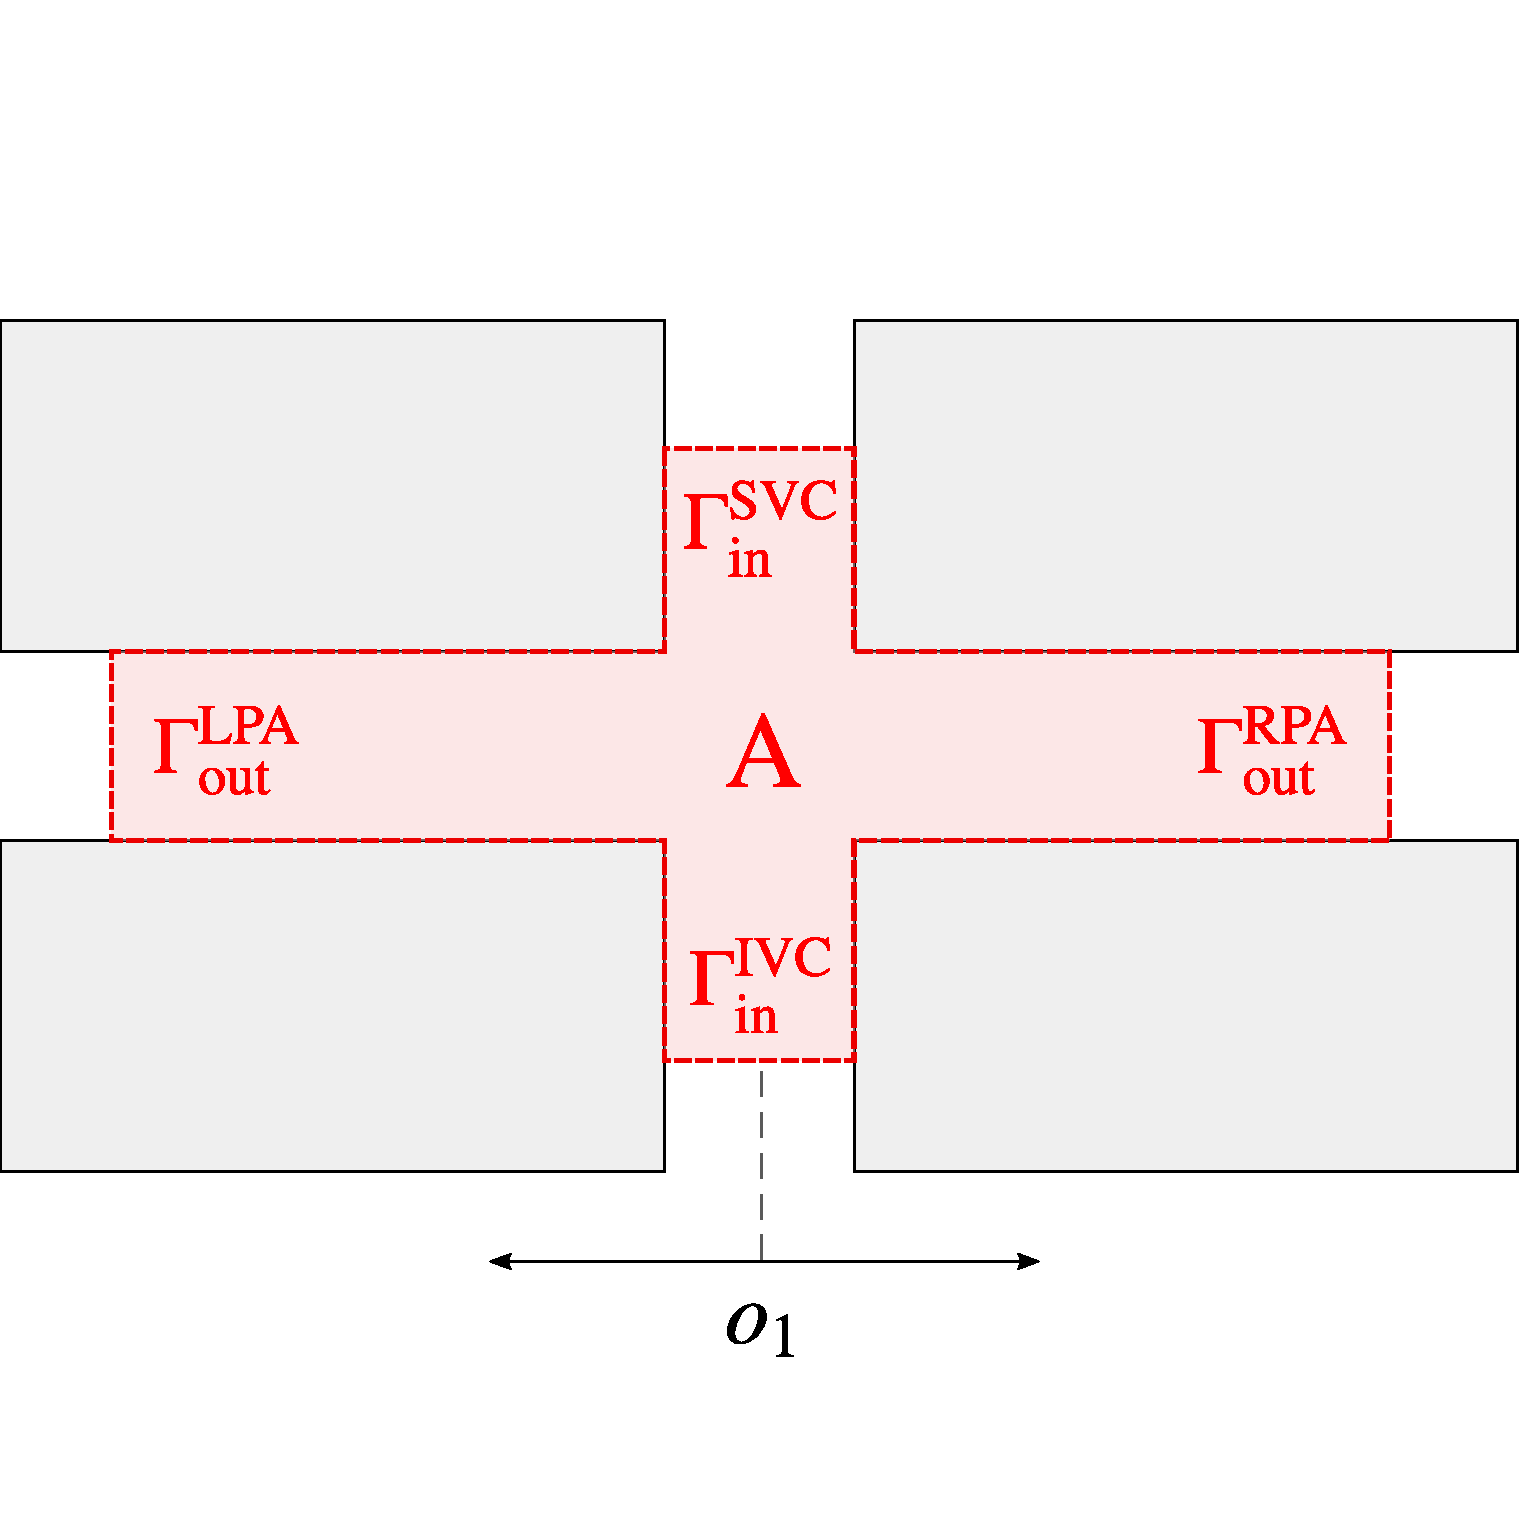
\includegraphics[width=0.91\textwidth, trim={0 0 0 0}]{figures/model1.pdf}
		\caption[Simplified Cylindrical Junction]{Schematic of Model 1: A simplified cylindrical junction with one degree of freedom, the horizontal offset of the IVC.}
		\label{fig:model1_schematic}
	\end{subfigure}\hfill%
	\begin{subfigure}{0.48\textwidth}
		\centering
		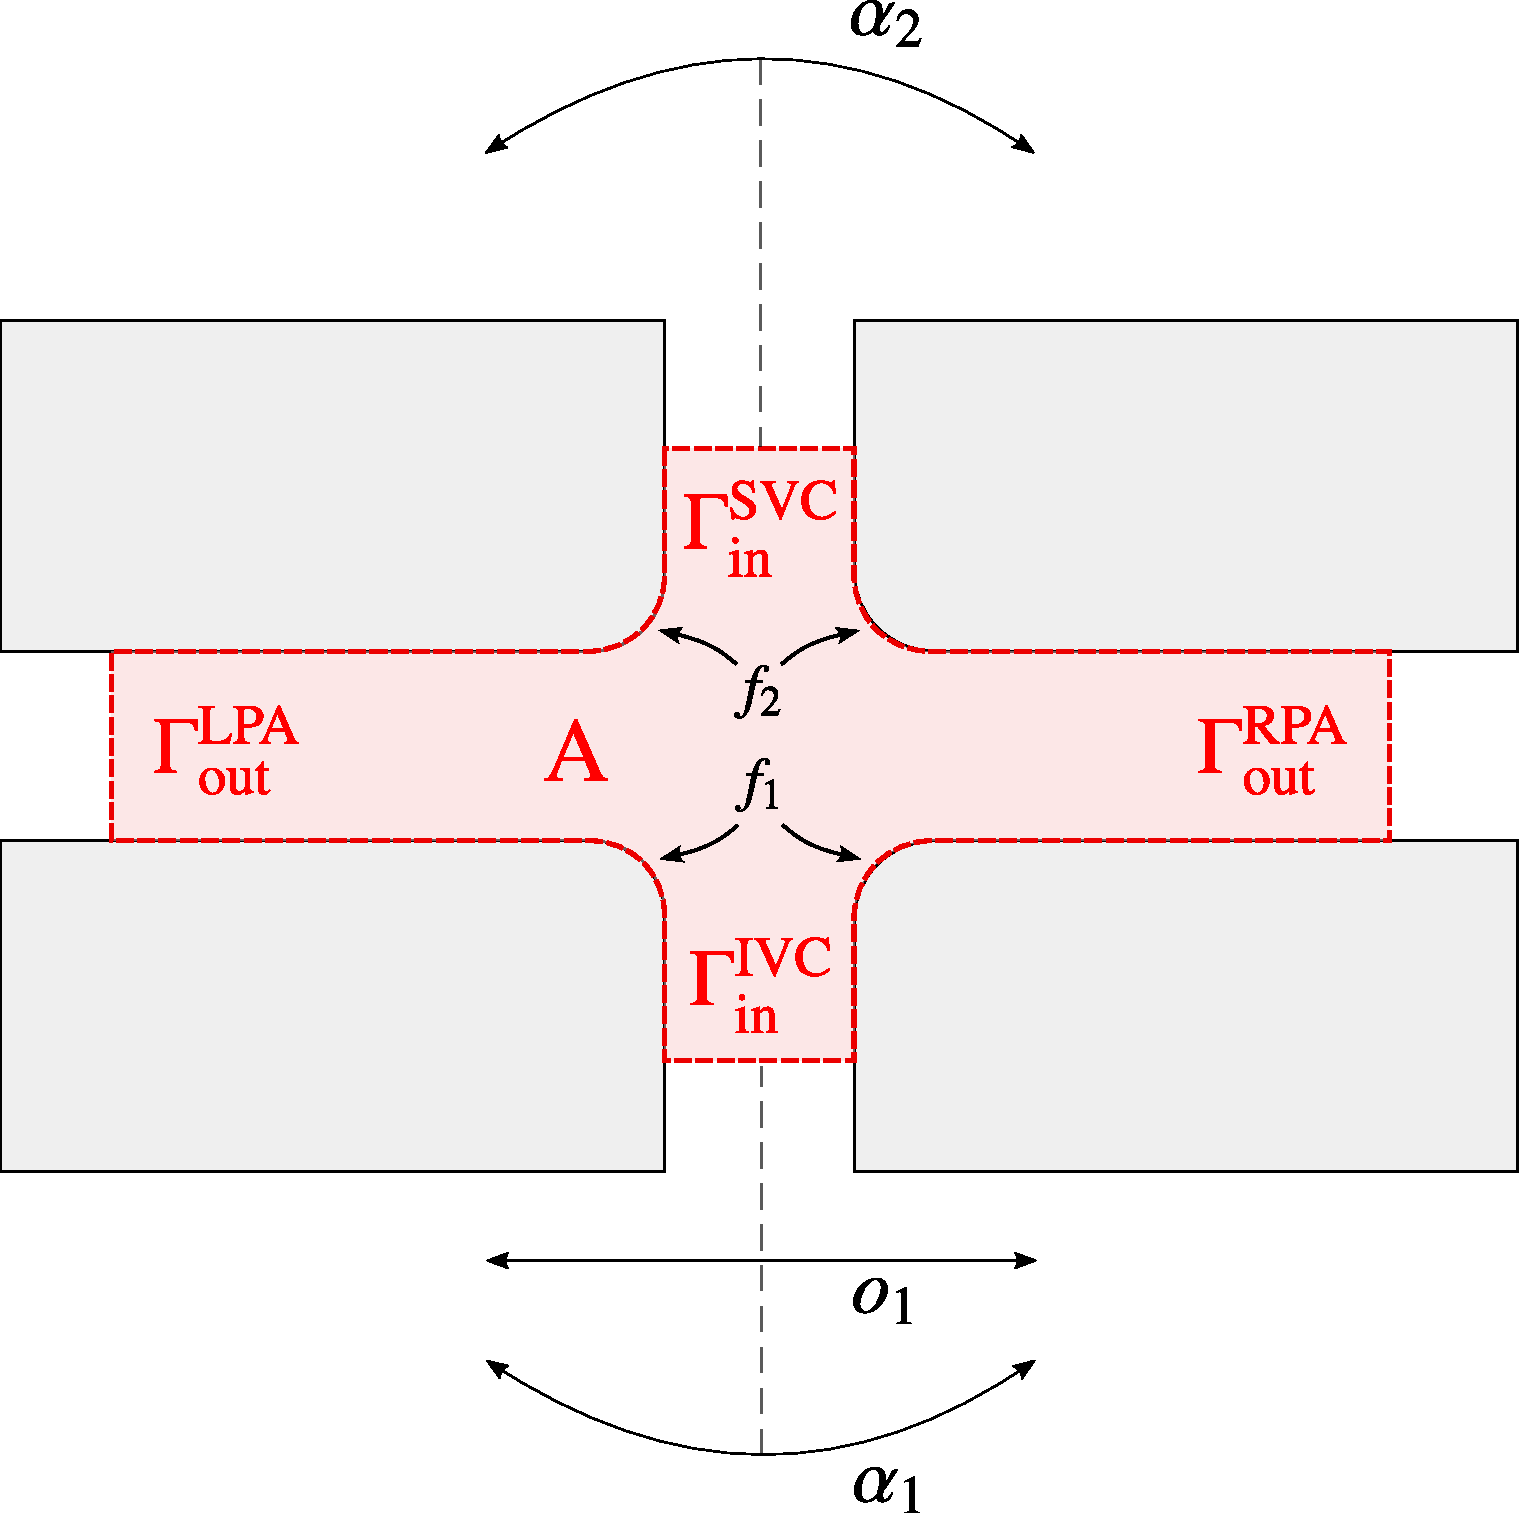
\includegraphics[width=0.91\textwidth]{figures/model2.pdf}
		\caption[Complex Geometric Model]{Schematic of Model 2: A more complex model introducing five degrees of freedom: IVC offset, connection angles and flaring.}
		\label{fig:model2_schematic}
	\end{subfigure}
	\vspace{4mm}
	\caption{Schematic illustrations of Model 1 and Model 2.}
	\label{fig:model schemas}
\end{figure}